\setcounter{step}{0}
%------------------------------------------
% information doc
\subsection{Marshmallow fondán}
\PrepTime{45}
\CookingTime{0}
\CookingTempe{0}
\TypeCooking{Príprava}
\NbPerson{4}
\Image{0 0 400 400}{images/pistkot_krem_salko} %style 2
%------------------------------------------

\begin{ingredient}
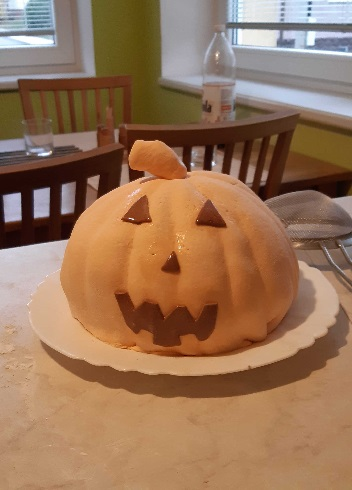
\includegraphics[height=5.5cm]{images/pistkot_krem_salko}
\def\portions{4}%
\textbf{{\normalsize Ingrediencie (\portions porcie):}}
%\vspace{0.5cm}
\begin{main}
	\item 200g marshmallow
	\item 1 ČL maslo
	\item 2 štipky kyseliny citrónovej
	\item 250g práškový cukor
\end{main}
\end{ingredient}
\begin{recipe}
\textbf{{\normalsize Príprava:}}
\begin{enumerate}

\item{Marshmallow, maslo a citrodeko dáme do misky a na minútu - dve do mikrovlnky. (Každých 15s premiešať.)}
\item{Pridávame preosiaty cukor. (Kým sa dá, miešame v miske)}
\item{Vyklopíme na dosku na preosiaty cukor, vyrobíme tuhšie cesto.}	
\item{Vyvaľkať a preniesť valčekom na tortu}

\end{enumerate}
\end{recipe}

\begin{notes}

\end{notes}
\clearpage	